\documentclass{beamer}

% for themes, etc.
\mode<presentation>
{ \usetheme{metropolis} }
%{ \usetheme{boxes} }

\usepackage{times}  % fonts are up to you
\usepackage{graphicx}

% these will be used later in the title page
\title{CHPC WLCG Tier2 Facility and SA Grid Operations}
\author{Sean Murray \\
    ALICE \\
    CHPC \\
    CSIR 
}
\date{October 6, 2016}

% note: do NOT include a \maketitle line; also note that this title
% material goes BEFORE the \begin{document}

% have this if you'd like a recurring outline
\AtBeginSection[]  % "Beamer, do the following at the start of every section"
{
\begin{frame}<beamer> 
\frametitle{Outline} % make a frame titled "Outline"
\tableofcontents[currentsection]  % show TOC and highlight current section
\end{frame}
}

\begin{document}

% this prints title, author etc. info from above
\begin{frame}
\titlepage
\end{frame}

\section{WLCG}

\begin{frame}
\frametitle{What is the WLCG}
\centering{
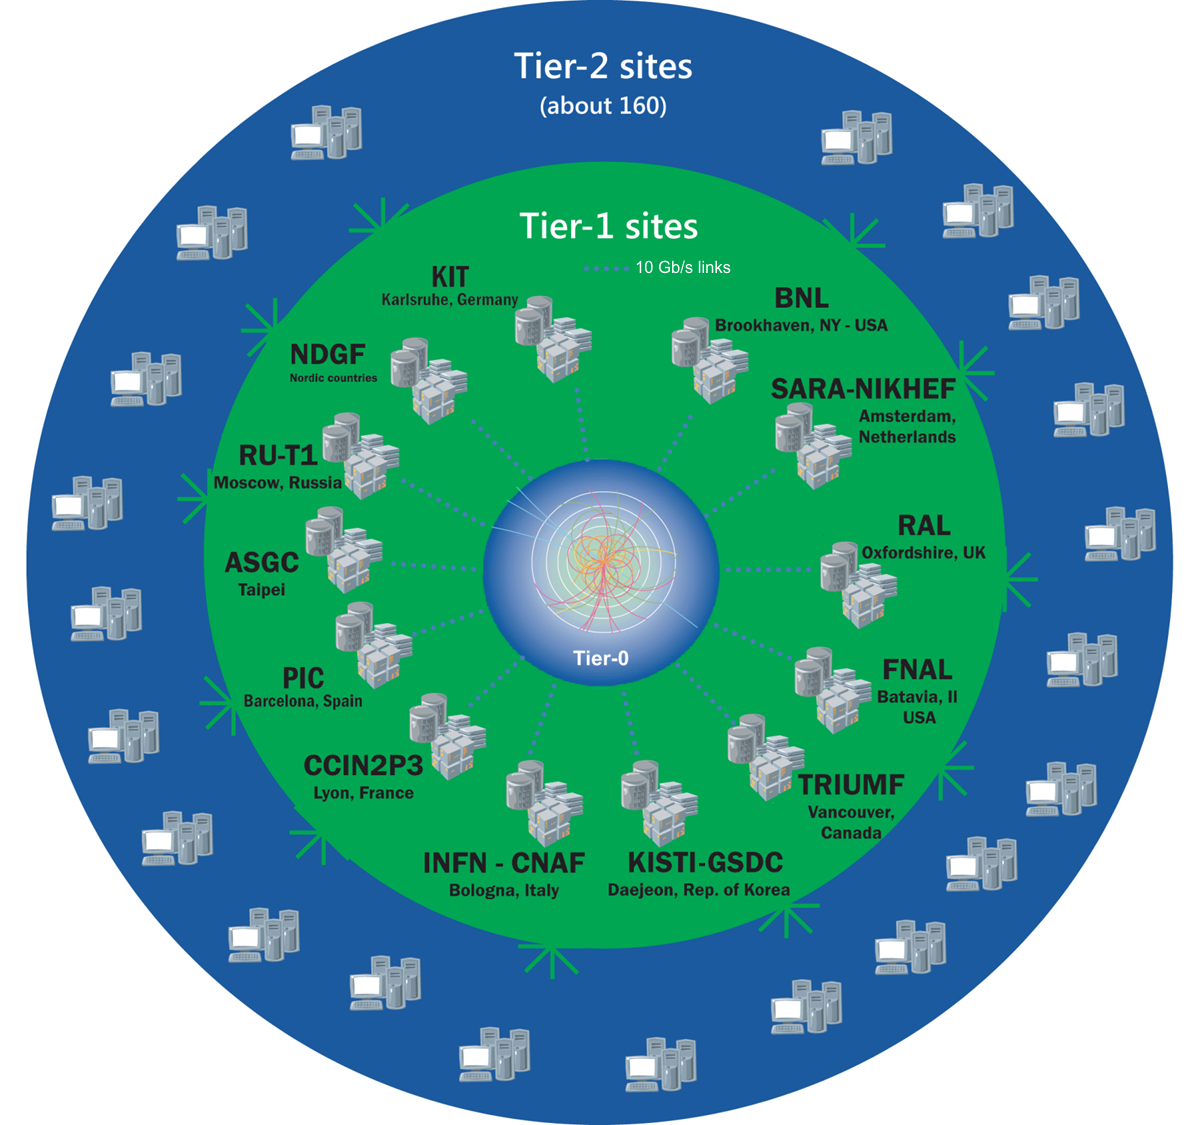
\includegraphics[scale=0.4]{WLCG-TiersJun14_v9.png}
}
\end{frame}
\begin{frame}
\frametitle{WLCG Map of Sites}
\centering{
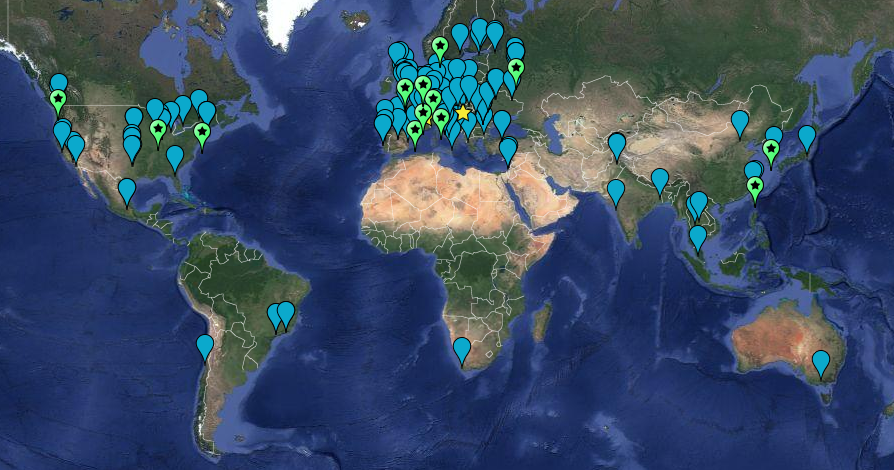
\includegraphics[scale=0.5]{WLCG-Sites.png}
}
\end{frame}

\begin{frame}
\frametitle{WLCG MOU Signed}
\begin{columns}[T] % align columns
\begin{column}{.48\textwidth}
  
\includegraphics[scale=0.45]{CHPCLogo.pdf}
  
\includegraphics[scale=0.45]{WLCGLogo.pdf}
\end{column}%
\begin{column}{.48\textwidth}
  \centering{
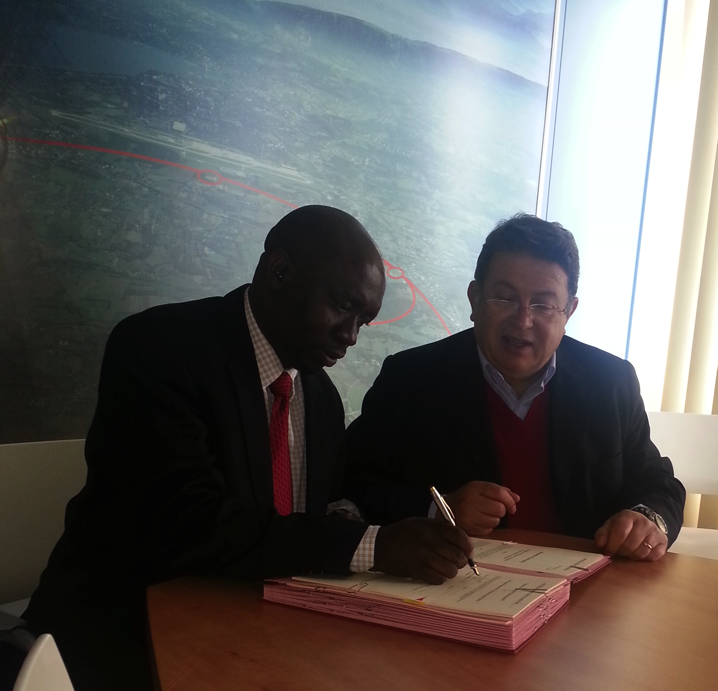
\includegraphics[scale=0.45]{WLCG-MOU_Signing.pdf}
} 
\end{column}%
\end{columns}  
\centering{28 April 2015}
\end{frame}

\begin{frame}
\frametitle{Commitments}
According to Tender :
\begin{itemize}
  \item ALICE 600 cores
  \item ATLAS 600 cores
  \item ALICE 400TB
  \item ATLAS 400TB
\end{itemize}
According to :
https://wlcg-rebus.cern.ch/apps/pledges/resources/
\begin{itemize}
  \item 6000 HEPSPEC06 cores (c. 560 of our cores)
  \item 100TB storage
  \item All ALICE.
  \item now equal ALICE and ATLAS (?)
\end{itemize}
\end{frame}

\begin{frame}
  \frametitle{Computing Infrastructure}
  \centering{
  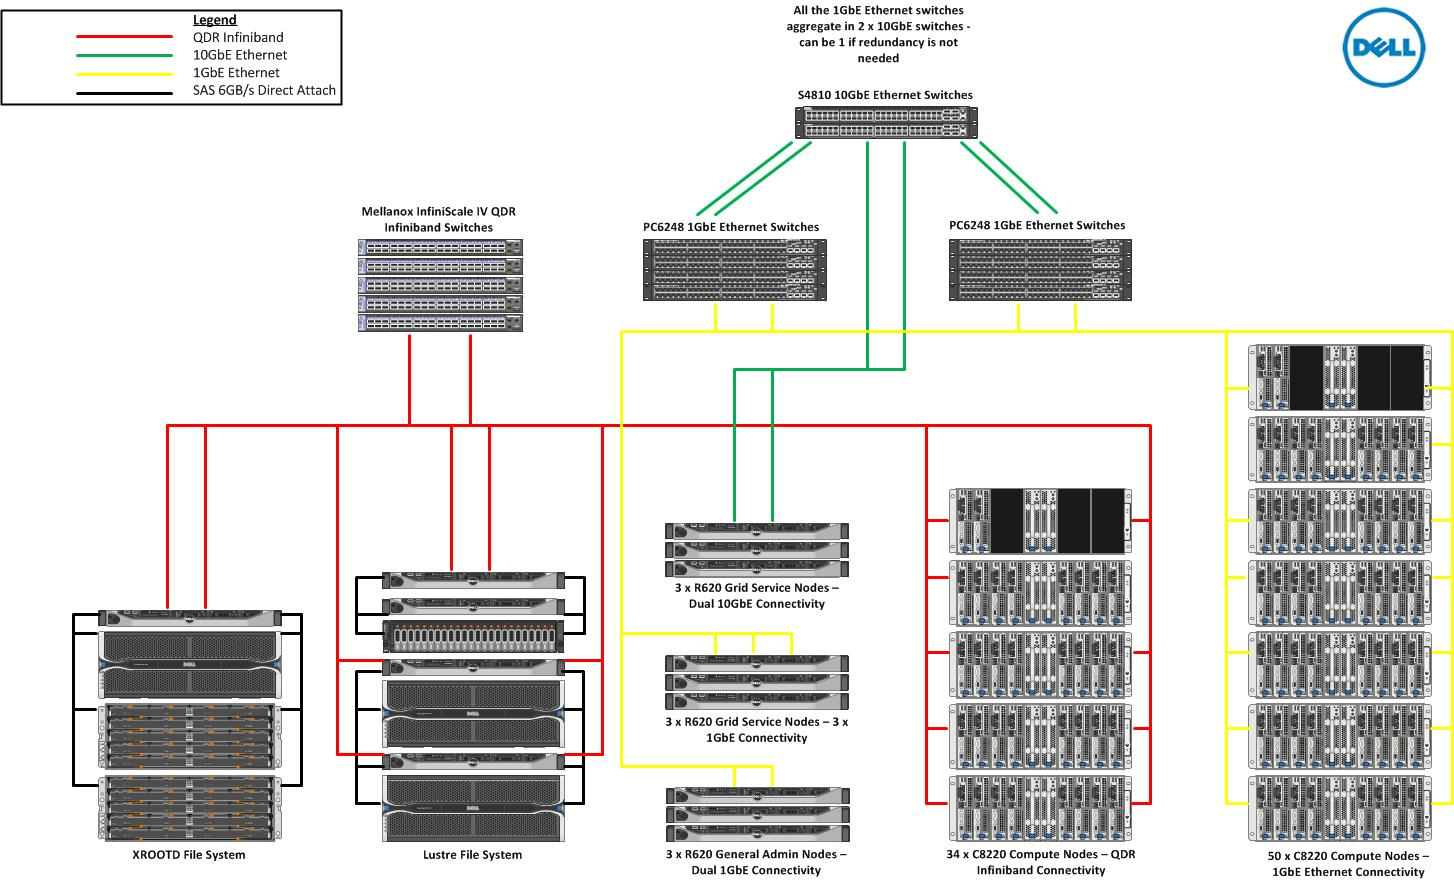
\includegraphics[scale=0.30]{CHPCConnectivityDiagram.jpg}
  }
\end{frame}

\begin{frame}
  \frametitle{Current hardware}
  \begin{itemize}
    \item 50 nodes of 48 cores 192GB RAM and 2x800TB of SSD, 1G ethernet
    \item 34 nodes of 48 cores 96GB RAM and 1TB SATA, FDR infiniband, 6 ``stolen''
    \item c.100TB of Lustre on the 34 nodes with FDR infiniband.
    \item 9 management servers, lower spec 
  \begin{itemize}
    \item compute element (head node,ce),
    \item storage element 2 redirectors, 2 storage nodes with direct attached multipath storage
    \item authentication, user interface (gone), monitoring, provisioning.
  \end{itemize} 
  \end{itemize}
\end{frame}

\begin{frame}
  \frametitle{Current Storage}
  \begin{itemize}
    \item 383TB EOS for ALICE, down from 440TB
    \item 252 TB EOS for ATLAS, down from 400TB
    \item 107 TB lustre for 34 nodes.
    \item 104 TB EMC for ATLAS, not going to be used.
    \item \color{red}{400TB ALICE}
    \item \color{red}{400TB ATLAS}
    \item \color{red}{400TB General EOS}
  \end{itemize}
Reduction in data sizes is due to reorganisation for reliability.
\end{frame}


\begin{frame}
  \frametitle{Current Performance}
\begin{itemize}
  \item 465k ALICE jobs in last year
  \item Avg concurrent jobs 1600, limited due to network..
  \item Data traffic consumed 70TB in and 60TB out in the last 3 months
\end{itemize}

\end{frame}

\begin{frame}
  \frametitle{Availability / Reliability}
  So who monitors us :
  \begin{itemize}
    \item WLCG
    \item EGI
    \item ALICE
    \item ATLAS
    \item me via zabbix/grafana and racktables
  \end{itemize}
There are a lot of eyes, ignoring the ones in this room.\\
\vspace{0.5cm}
\centering{
\begin{tabular}{|c|r|r|r|}
  Function     &  July & August & September \\ \hline 
  Availability &  100   &  100     & 100\\ \hline
  Reliability  &  100    &  100    & 100\\ \hline
\end{tabular}
\\I am soooo going to regret this slide !
}\\
\vspace{0.5cm}
\end{frame}

\begin{frame}
  \frametitle{Grafana ALICE}
  \centering{
  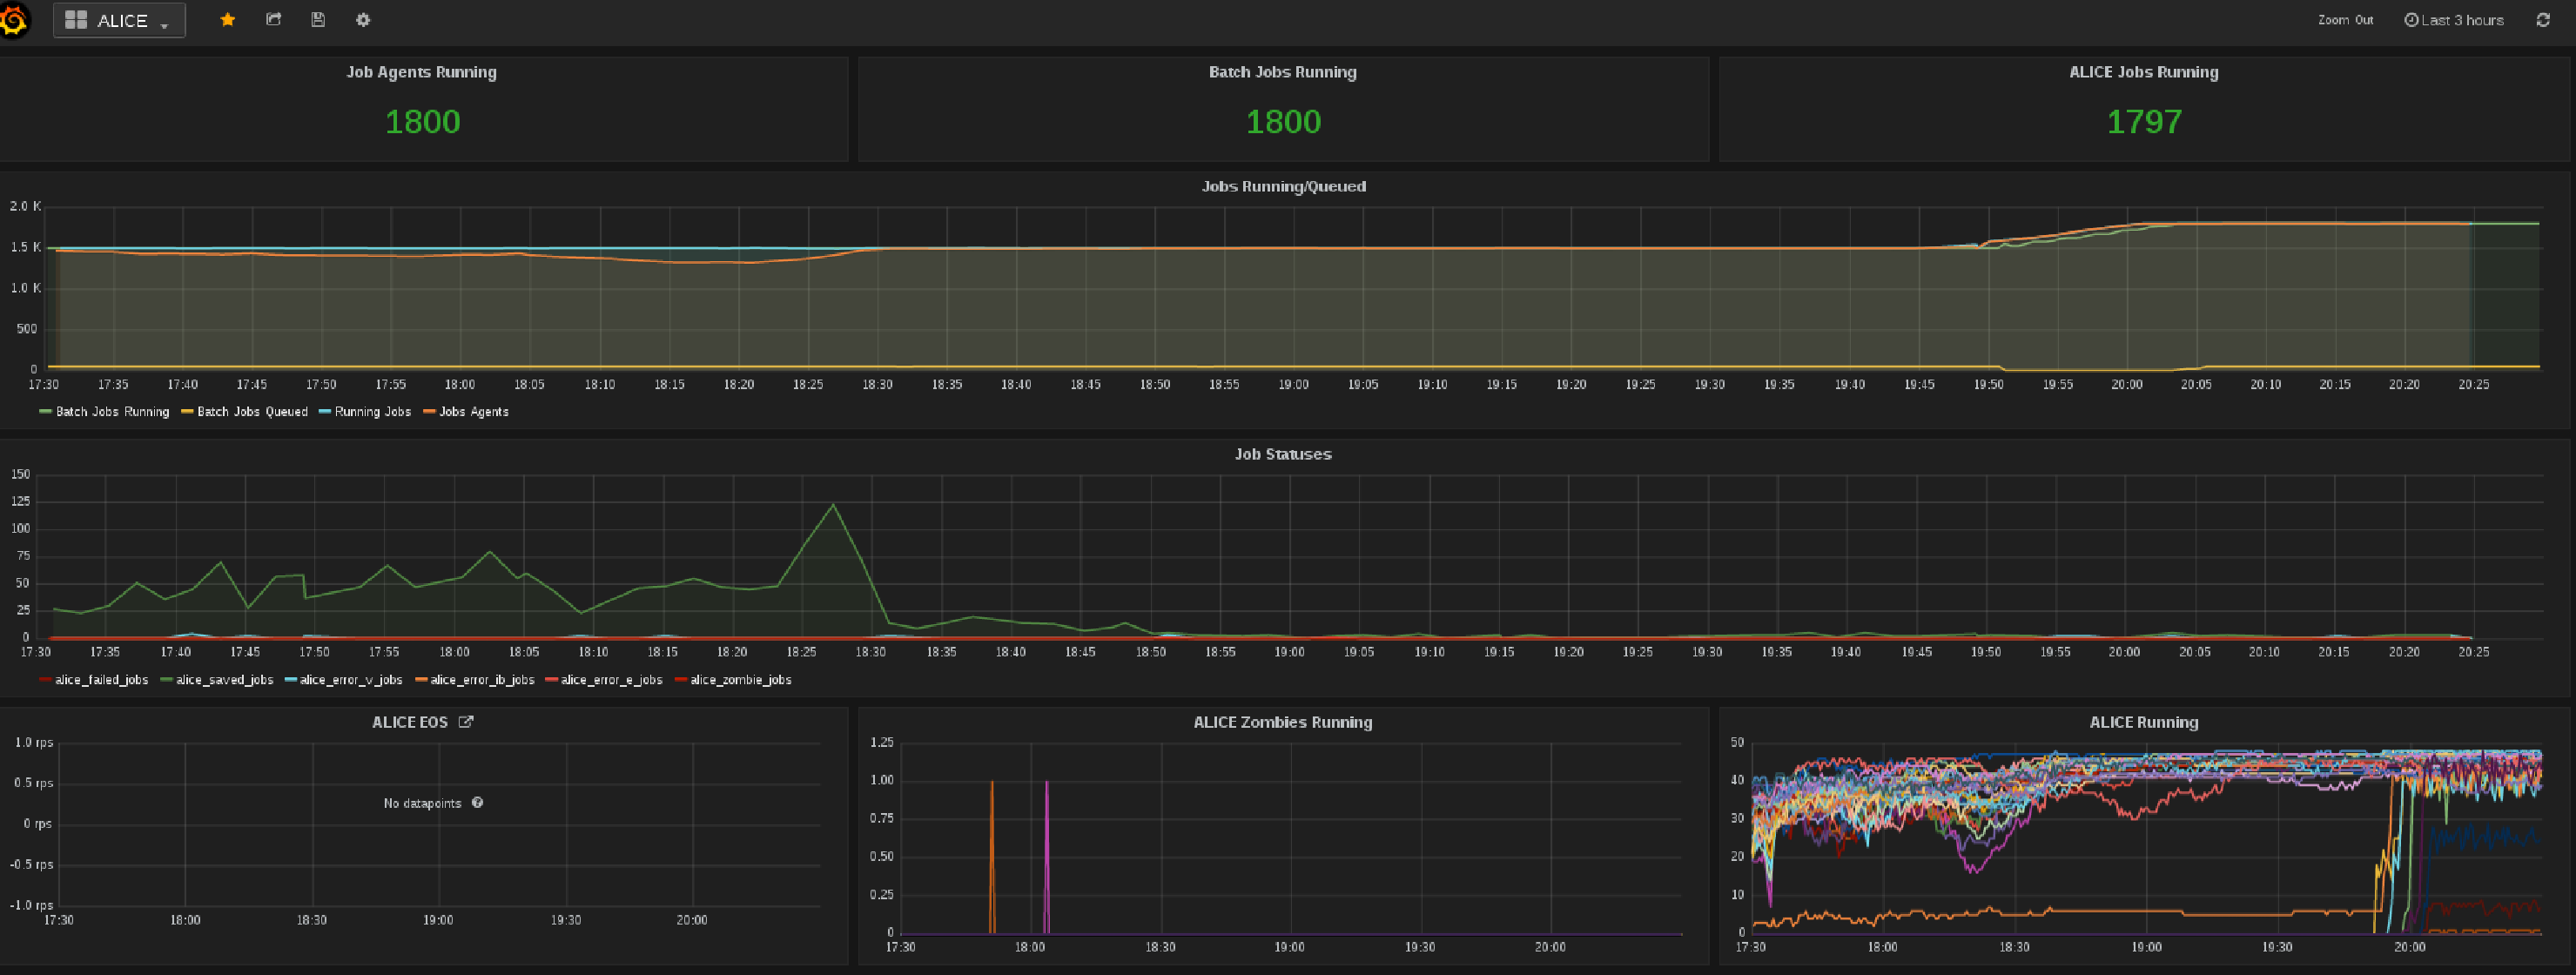
\includegraphics[scale=0.25]{ALICEProcessing-Grafana.pdf}
  }\\
  This is currently being expanded to pull in more from MonaLisa, and more experiment and storage specific
  metrics to help to trivialy diagnose and forewarn problems.
\end{frame}

\begin{frame}
  \frametitle{Our Data's Scenic Tour}
  \centering{
  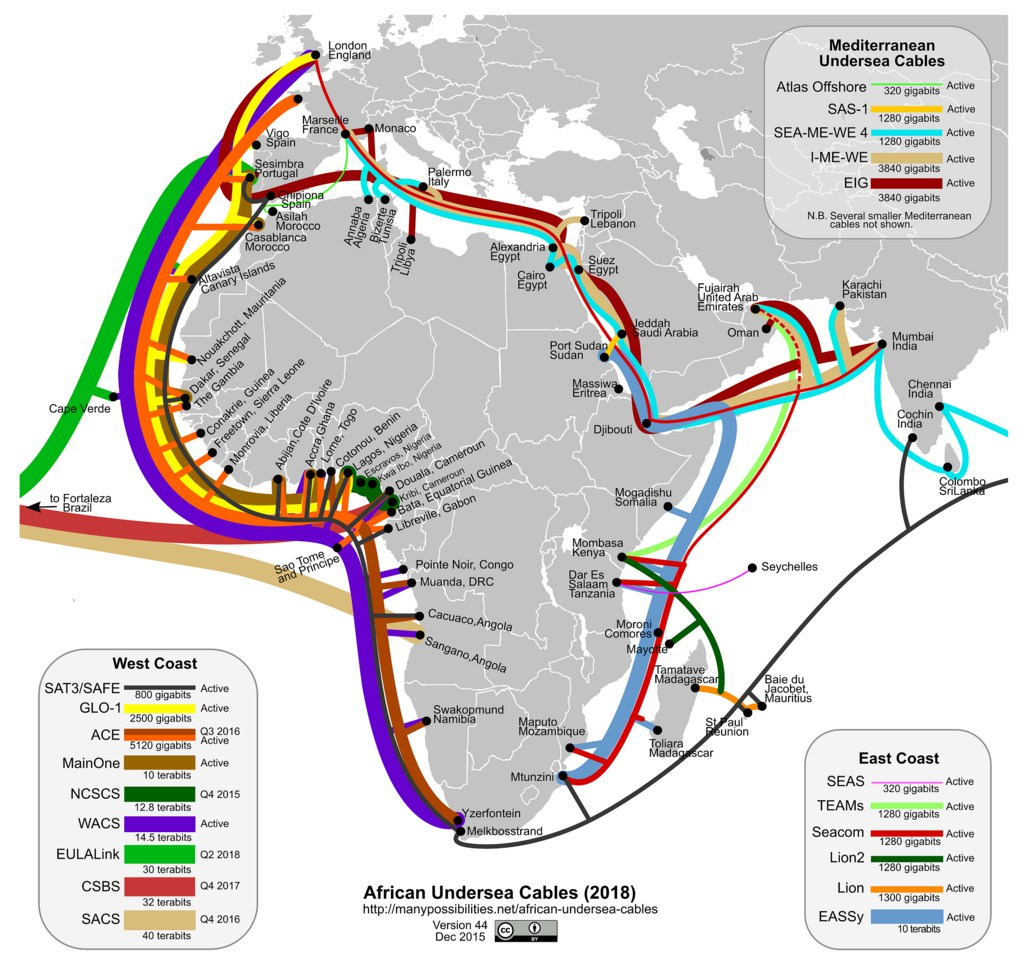
\includegraphics[scale=1]{african_undersea_cables.jpg}
  }
\end{frame}

\begin{frame}
  \frametitle{Tier2 Processing}
  \begin{itemize}
    \item ATLAS processing direct std batch jobs.
    \item ALICE processing, job agents and leave it to central services, vobox.
    \item ops jobs fail due to starvation from alice. currently a dedicated machine
    \item all software is distributed via cvmfs, both experiments.
    \item ALICE has something similar to code-rade, an entire ecosystem of modules, versions, builds, etc.
    \item still no official validation on CC7.
  \end{itemize}
\end{frame}

\begin{frame}
  \frametitle{Tier2 Storage operations}
  Thankfully both experiments use xrootd.
  \begin{itemize}
    \item ALICE has its own authentication system, controlled centrally from CERN.
    \item ALICE has one big block of storage.
    \item ATLAS uses grid pool accounts, more standard grid.
    \item ATLAS has various storage's on site, cut up locally.
    \item ATLAS on puppet, ALICE will go on puppet when upgraded.
  \end{itemize}
\end{frame}

\begin{frame}
  \frametitle{Philosophy}
  \begin{itemize}
    \item Keep It Simple Simpleton.
    \item Only use liberally licensed software.
    \item Stand on whom evers shoulders I can.
    \item I dont want to do sys admin, I dont enjoy it.
    \item Abstract sys admin to a Software Engineering problem.
    \item Let me get back to the things that I enjoy ALICE O2 and HLT which I enjoy, computational physics..
  \end{itemize}
\end{frame}

\begin{frame}
  \frametitle{Simple Solution}
  Switch everything off for 4 or 5 months while i redo \bf{everything}
\end{frame}

\begin{frame}
  \frametitle{the plan}
  \begin{itemize}
    \item Keep site up and processing maintaing our Tier 2 status.
    \item incrementally replace systems.
    \item the return of 28 grid nodes, on infiniband, a place to test configurations when batch is ``free''.
  \end{itemize}
\end{frame}


\begin{frame}
  \frametitle{Improvements}
  \begin{itemize}
    \item Fixed ALICE error rates, mostly.
    \item ALICE concurrent jobs from 700 to 1800.
    \item max out bandwidth now regularly.
    \item ATLAS running pilot jobs. 
    \item Storage cleaned up and reduced.
    \item New storage quoting
    \item Plan in place to overhaul, and being tested.
    \item Work defined to Redo entire internal network.
  \end{itemize}

\end{frame}
\begin{frame}
  \frametitle{upgrades}
  \begin{itemize}
    \item attempts to delay till CC7 validation have failed.
    \item Puppify, to auto site deployment, r10k an issue.
    \item Transition to foreman from xcat.
    \item upgrade monitoring server to zabbix3, via docker this time.
    \item Rewire whole network, re-power to monitored pdu, and monitor all.
    \item Add inherent redundancy into 10G interfaces on ce,se,se2.
    \item Reinstall while TRYING to keep A/R. problems are vobox and ce. 
    \item Storage, we need an additional 750TB for ALICE and ATLAS just to maintain Tier2.
  \end{itemize}
\end{frame}
\begin{frame}
  \frametitle{Transparency}
  Historically this has not been great, so \ldots
  \begin{itemize}
    \item Federated logins to zabbix and grafana, i.e. You
    \item All code on github in line with AAROC
    \item All issues PUBLIC on github, this has been a serious uhming and ahring session.
    \item Still have GGUS for normal tickets.
    \item Some training on the user analysis facility (hopefully online)
    \item A couple of things remain private like network diagrams, obviously, and passwords. github encrypted repos (todo)
    \item AAROC slac channels.
  \end{itemize}
\end{frame}
\begin{frame}
  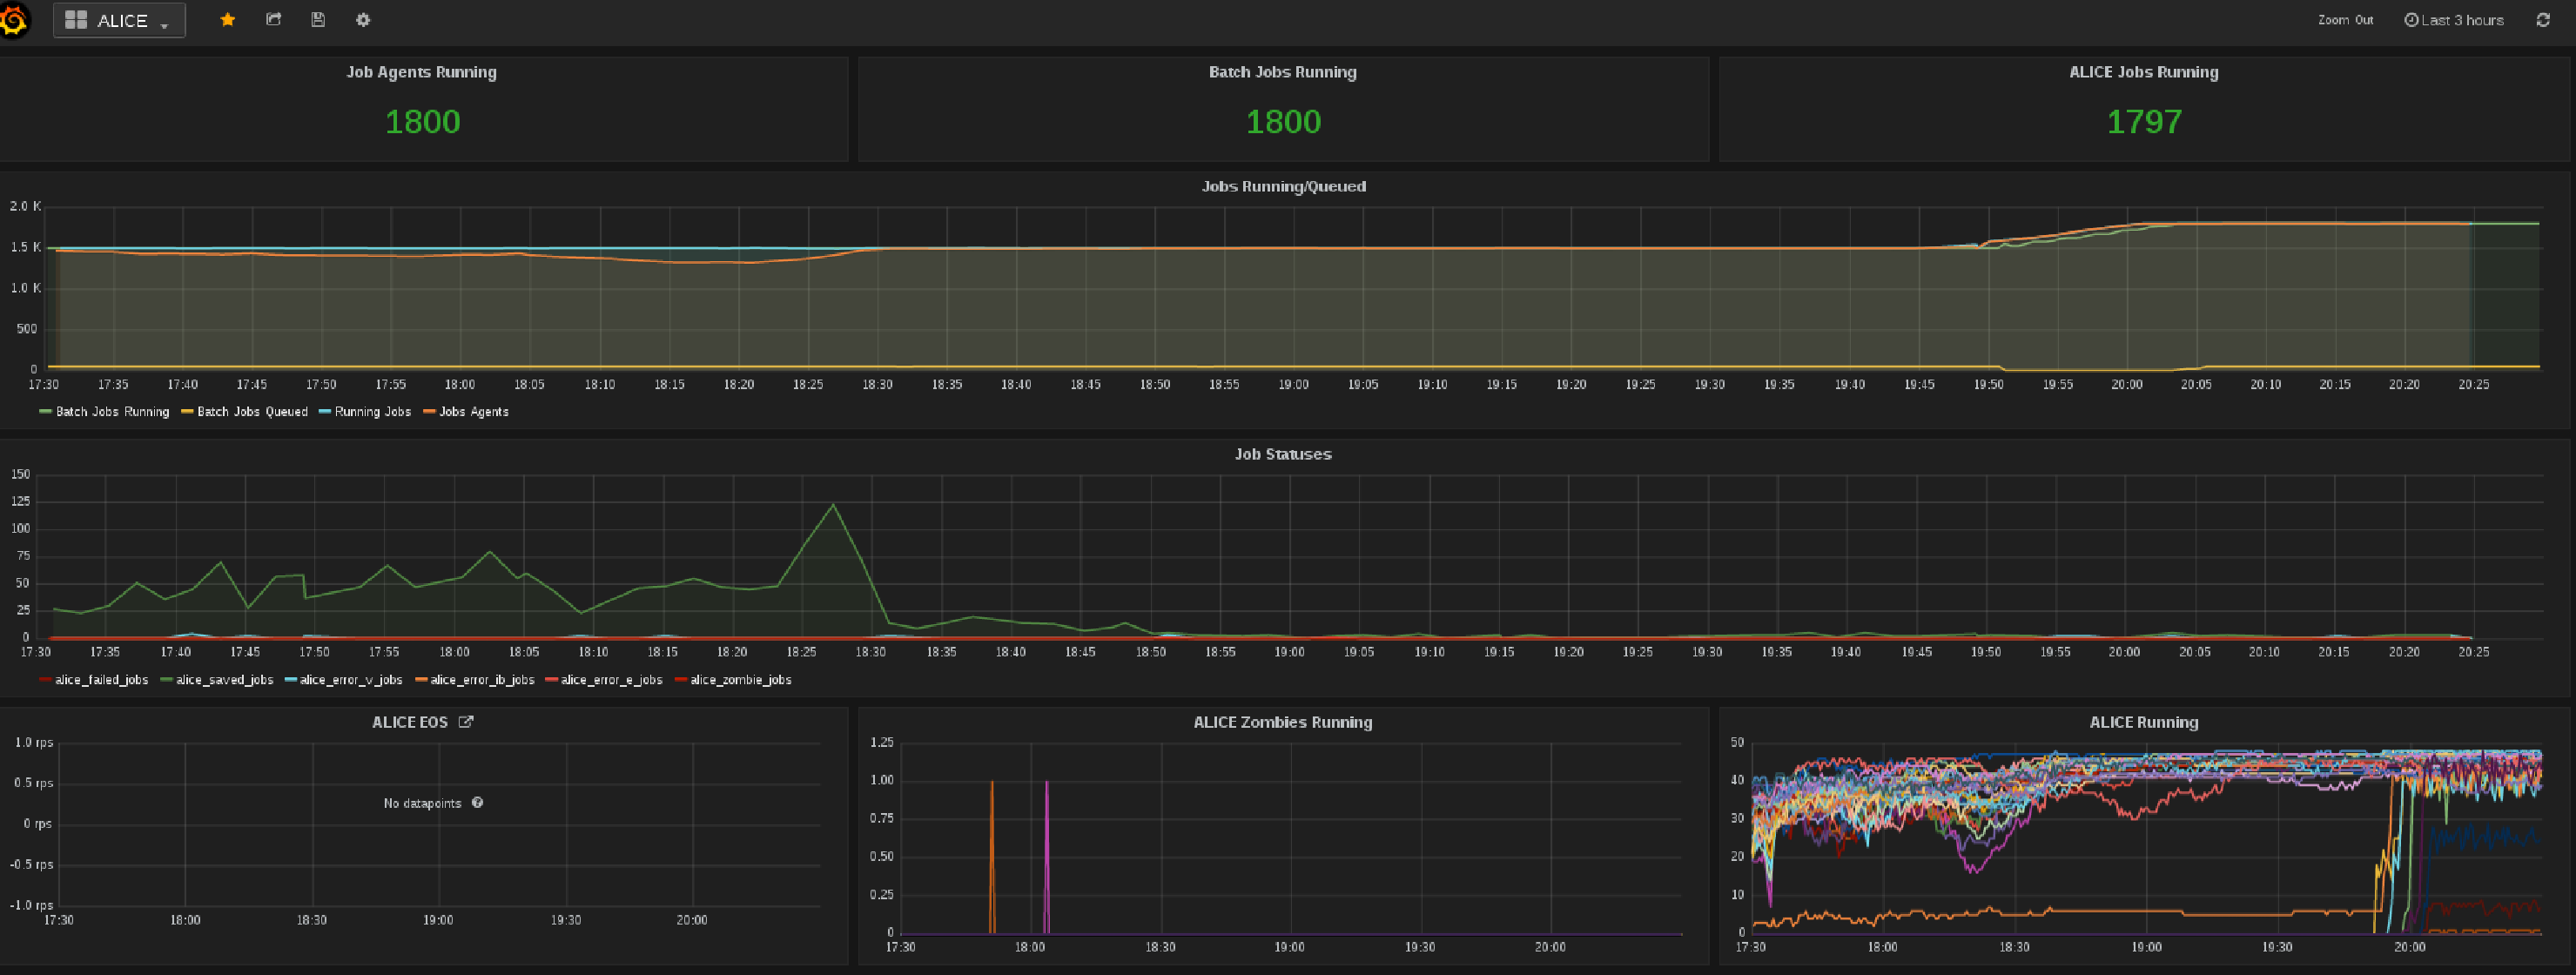
\includegraphics[scale=0.25]{ALICEProcessing-Grafana.pdf}\\
  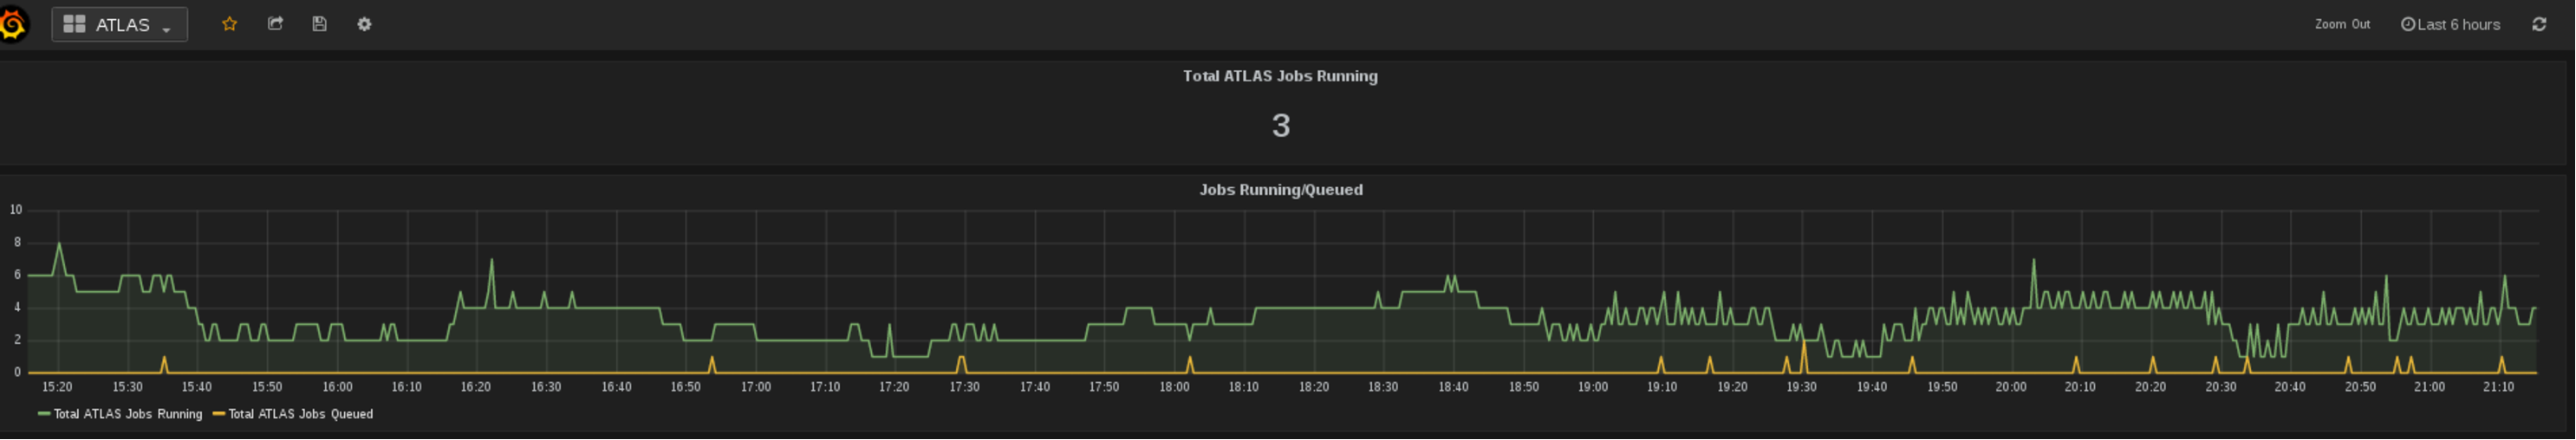
\includegraphics[scale=0.25]{ATLASProcessing-Grafana.pdf}\\
  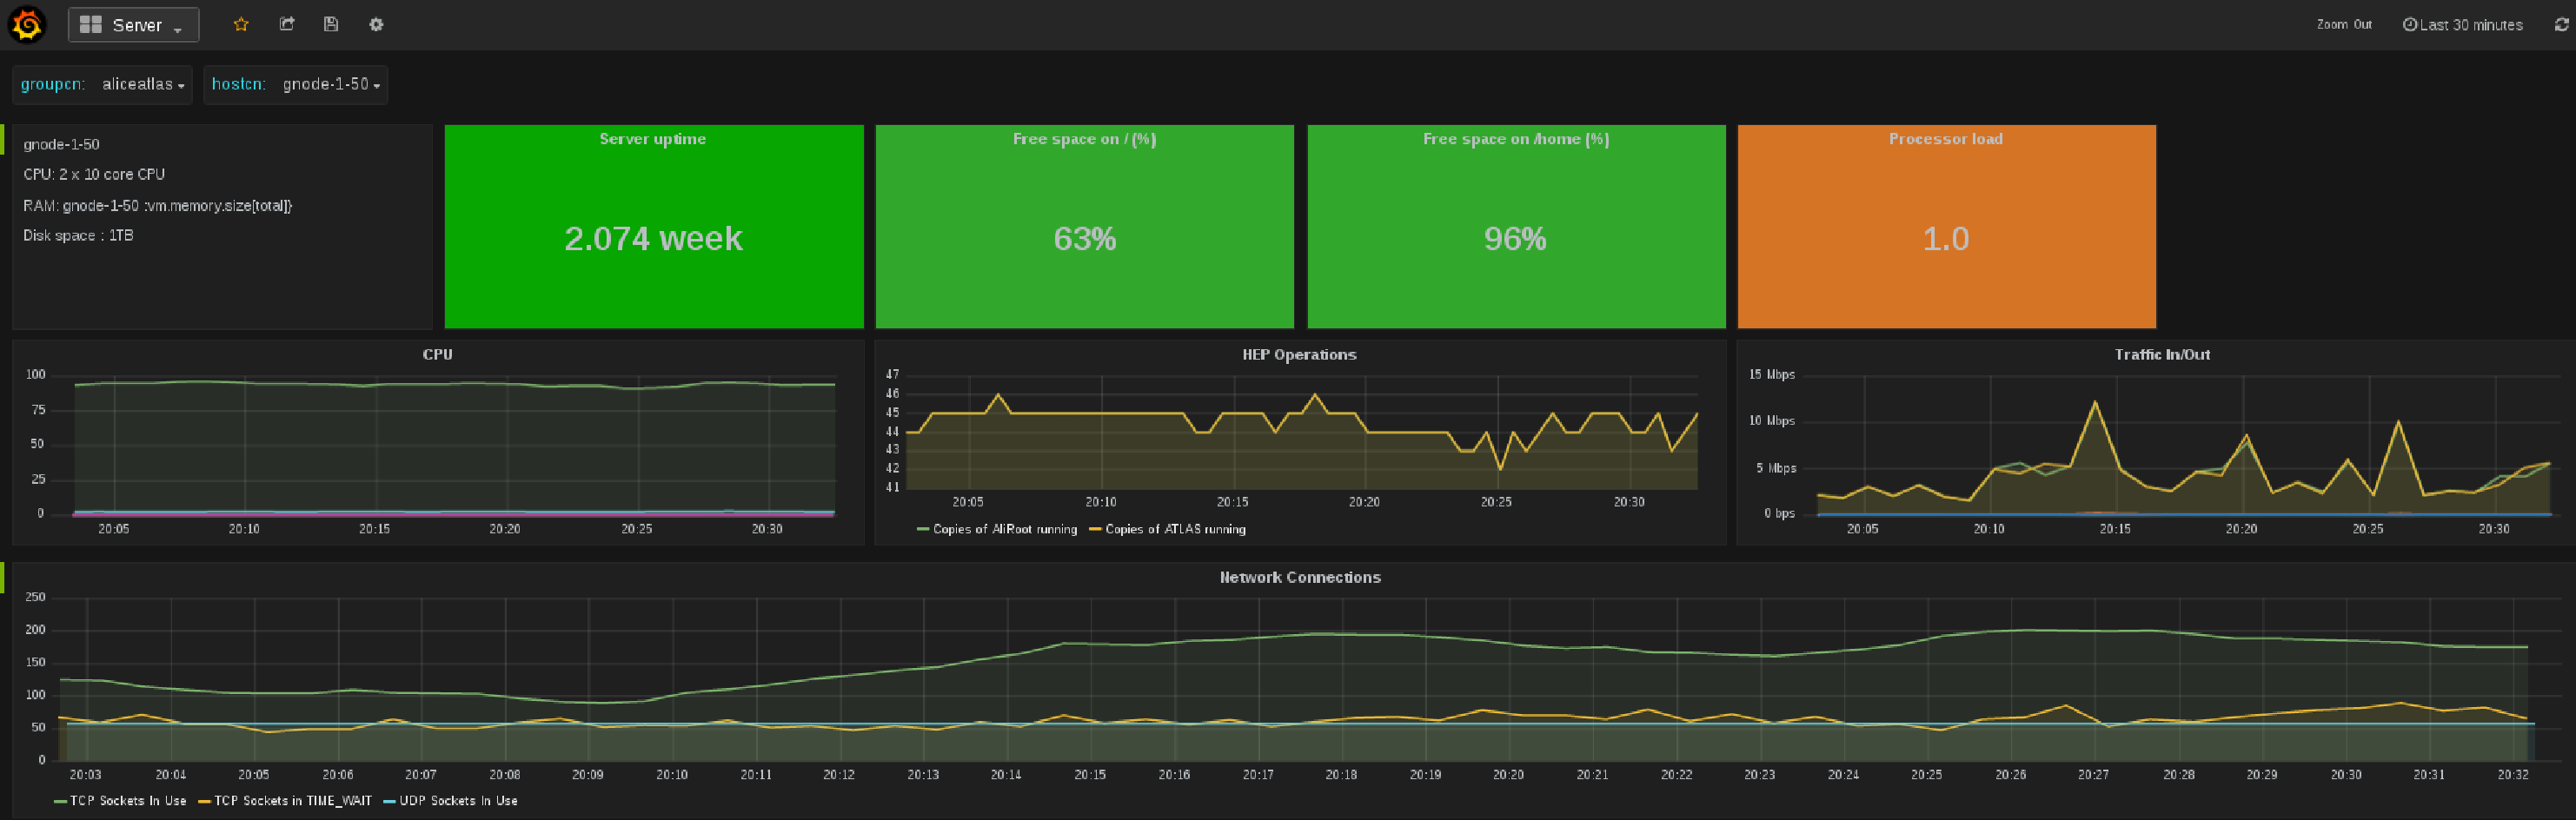
\includegraphics[scale=0.25]{Server50-Grafana.pdf}\\
  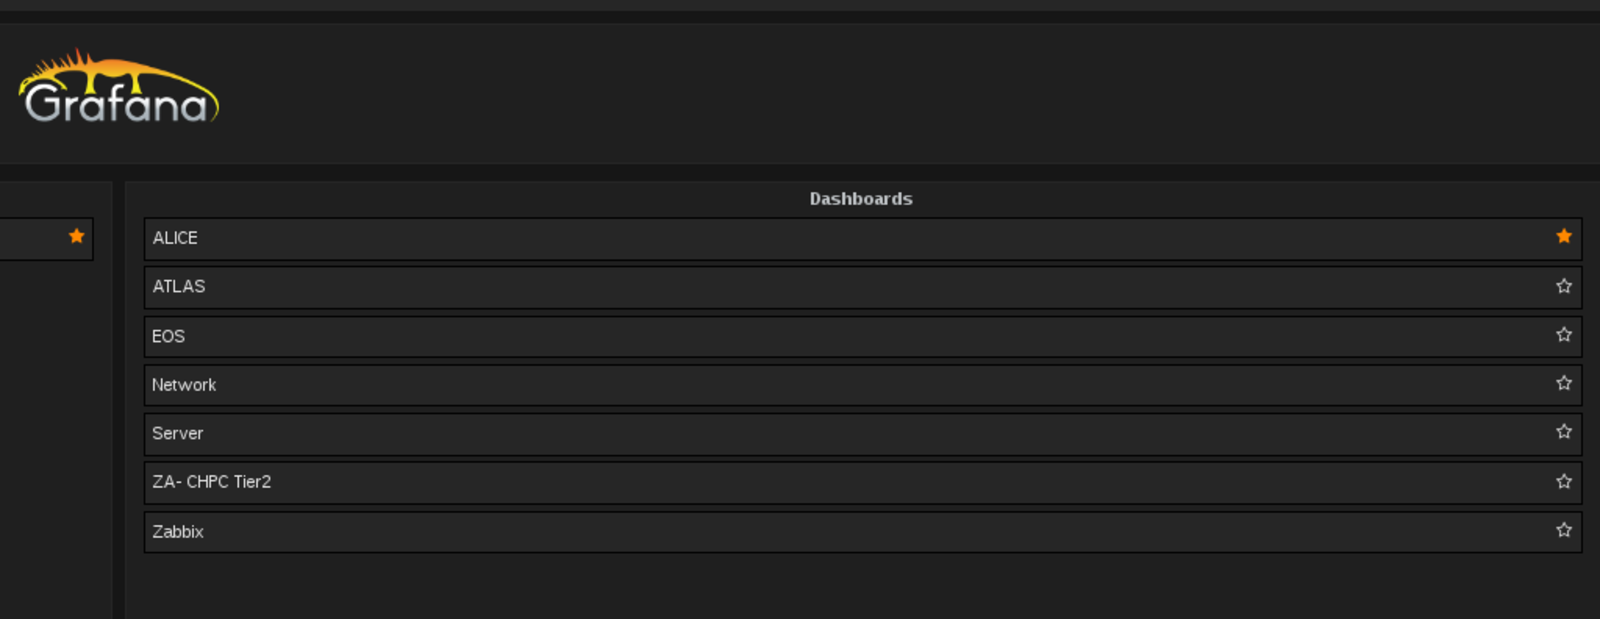
\includegraphics[scale=0.25]{GrafanaMenu.pdf}
\end{frame}


\section{SAGrid, user analysis}
\begin{frame}
\frametitle{28 nodes}
July 28 of the 34 nodes came back for SAGrid and HEP user analysis.
\begin{itemize}
  \item Go back to SAGrid to support anybody on SAGrid VO.
  \item HEP user analysis, based on federated identities, no user account admin.
  \item either HEP user supplies their own eco system with job or build their custom ecosystem via code-rade.
  \item code based on CODE-RADE, or LHC experiments.
  \item HLT replica for me and others. (no gpu)
  \item O2 dev for O2 development with dds/mesos/pbs. (no gpu/fpga)
  \item \color{red}{Local Storage for users, eos and lustre.}
  \item 24/4 sl6/centos7 in prep for container migration.
\end{itemize}
\end{frame}

\begin{frame}
  \frametitle{deployment/provisioning}
  Foreman \ldots
  \begin{enumerate}
    \item deployment
    \item configuration, puppet, chef, salt, ansible.
    \item monitoring.
  \end{enumerate}
  Not using the fully integrated puppet/foreman as i prefer to be 
  tool agnostic, or at least strive for it.
\end{frame}


% alibuild sim to code-rade all built in cvmfs or use scripts to build own systme environment.
\begin{frame}
  \frametitle{puppet}
  A method/system to maintain a system in a known state.\\
  hiera, a key value store used by puppet.\\
  We store all site specific information in hiera, tightly integrated into puppet..
\end{frame}

\begin{frame}
\frametitle{AAROC Devops and r10k}
\begin{itemize}
  \item r10k branches are mapped to environments (dev, testing, production).\\
  \item Cant be under AAROC, so chpctier2, production branch will be synced to aaroc/devops/chpc.\\
  \item 3 branches, dev, testing and production, currently only use production.
\end{itemize}
\end{frame}

\begin{frame}
  \frametitle{Testing}
  Devops requires some form of automated testing.
  \begin{itemize}
    \item Unit testing via rspec.
    \item Function testing.
    \item Fact testing.
    \item System testing.
  \end{itemize}
\end{frame}

\begin{frame}
  \frametitle{Monitoring}
  \begin{itemize}
    \item zabbix
    \item grafana on zabbix.
    \item racktables with zabbix link.
    \item foreman
    \item monalisa
    \item have singular sources of authority. idrac mostly.
  \end{itemize}
\end{frame}

\begin{frame}
  \frametitle{network}
  put in pics from other doc of old and new.
  ipmi interfaces in, monitor all including pdu's
  direct dual 10G links to interwebs.
\end{frame}

\begin{frame}
  \frametitle{bandwidth}
  explain test and results.
\end{frame}



\section{Backup Slides}

\begin{frame}
  \frametitle{LHCOPN}
  \centering{
  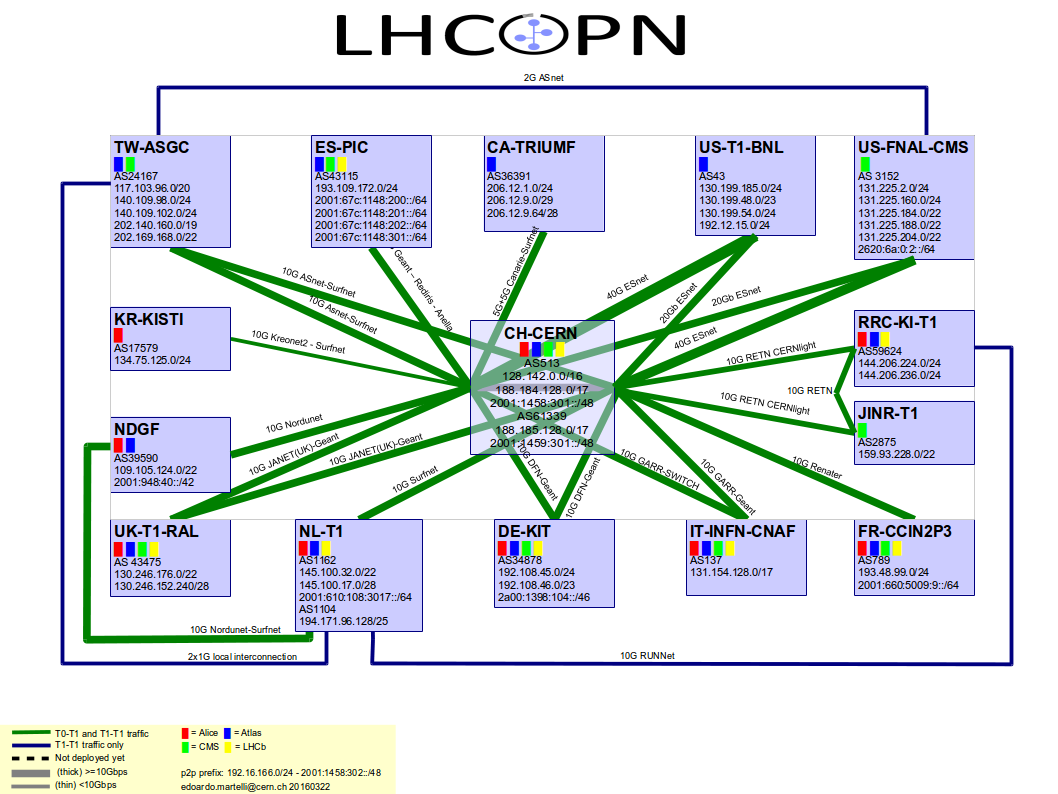
\includegraphics[scale=0.4]{map-lhcopn.png}
  }
\end{frame}

\begin{frame}
  \frametitle{IOU table}
  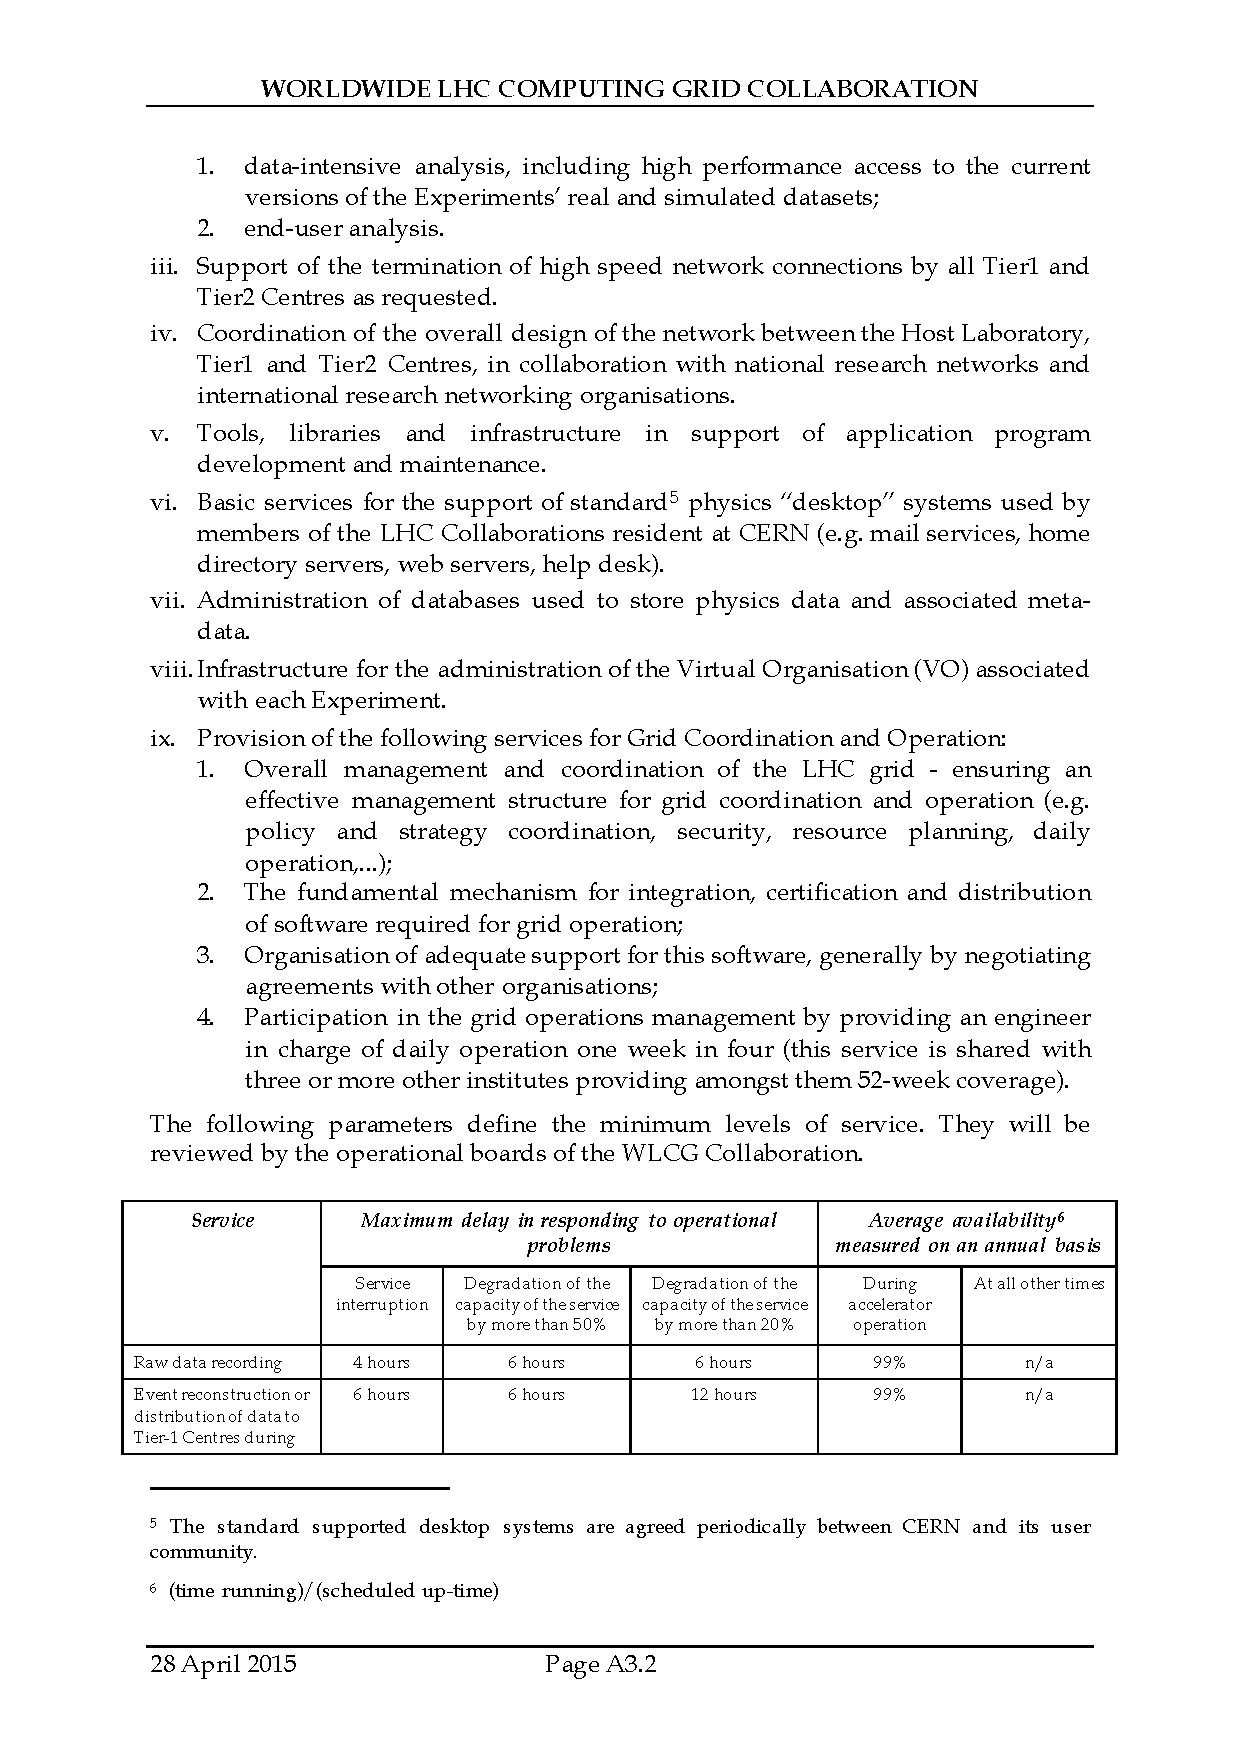
\includegraphics[scale=0.51,trim={1cm 5cm 1cm 18cm},clip]{mou_page23.pdf}\\
  
\includegraphics[scale=0.51, trim={1cm 10cm 1cm 2cm},clip]{mou_page24.pdf}
\end{frame}

\begin{frame}
  \frametitle{mou table}
  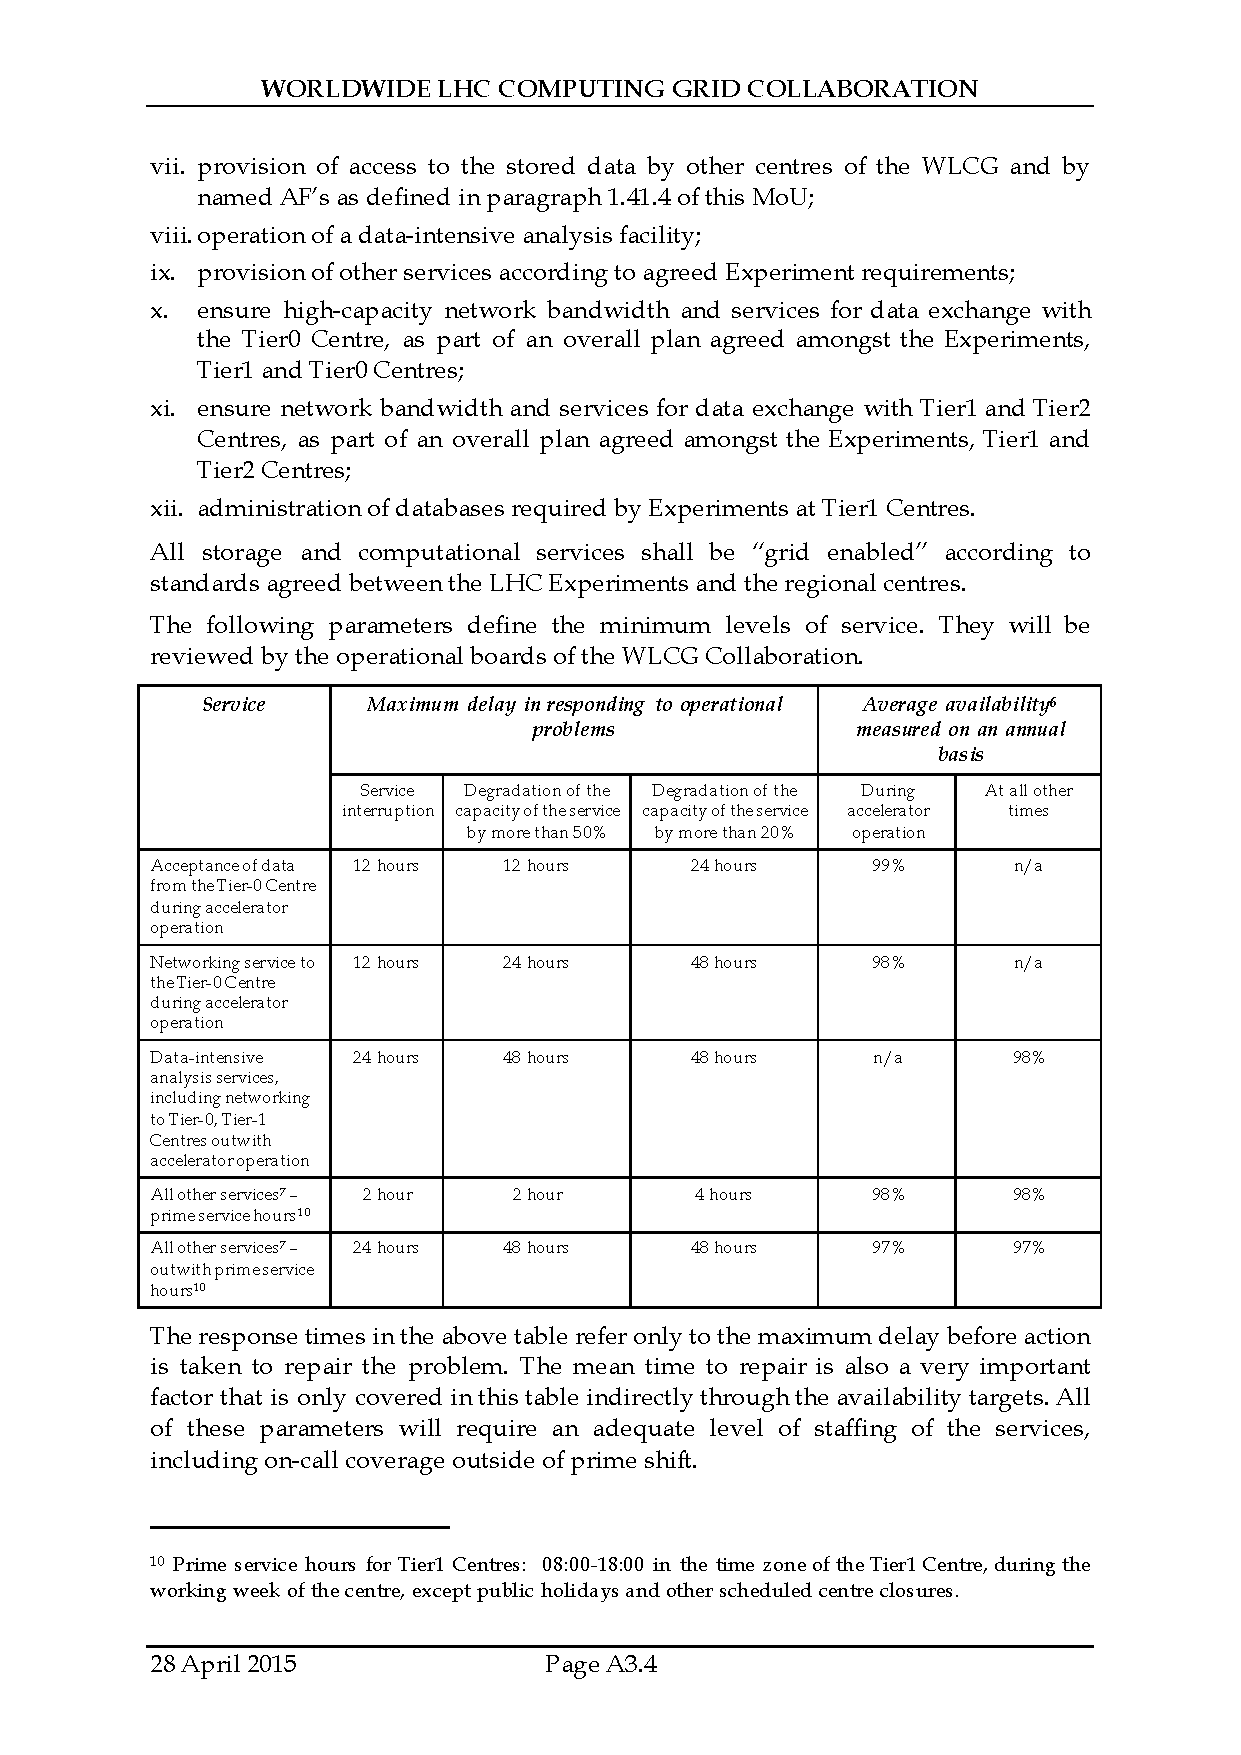
\includegraphics[scale=0.5, trim={1cm 7cm 1cm 11cm},clip]{mou_page25.pdf}
\end{frame}

\end{document}
